%%% The main file. It contains definitions of basic parameters and includes all other parts.

%% Settings for single-side (simplex) printing
% Margins: left 40mm, right 25mm, top and bottom 25mm
% (but beware, LaTeX adds 1in implicitly)
\documentclass[12pt,a4paper]{report}
\setlength\textwidth{145mm}
\setlength\textheight{247mm}
\setlength\oddsidemargin{15mm}
\setlength\evensidemargin{15mm}
\setlength\topmargin{0mm}
\setlength\headsep{0mm}
\setlength\headheight{0mm}
% \openright makes the following text appear on a right-hand page
\let\openright=\clearpage

%% Settings for two-sided (duplex) printing
% \documentclass[12pt,a4paper,twoside,openright]{report}
% \setlength\textwidth{145mm}
% \setlength\textheight{247mm}
% \setlength\oddsidemargin{14.2mm}
% \setlength\evensidemargin{0mm}
% \setlength\topmargin{0mm}
% \setlength\headsep{0mm}
% \setlength\headheight{0mm}
% \let\openright=\cleardoublepage

%% Generate PDF/A-2u
\usepackage[a-2u]{pdfx}

%% Character encoding: usually latin2, cp1250 or utf8:
\usepackage[utf8]{inputenc}

%% Prefer Latin Modern fonts
\usepackage{lmodern}

%% Further useful packages (included in most LaTeX distributions)
\usepackage[titletoc]{appendix}
\usepackage{amsmath}        % extensions for typesetting of math
\usepackage{amsfonts}       % math fonts
\usepackage{amsthm}         % theorems, definitions, etc.
\usepackage{bbding}         % various symbols (squares, asterisks, scissors, ...)
\usepackage{bm}             % boldface symbols (\bm)
\usepackage{graphicx}       % embedding of pictures
\usepackage{fancyvrb}       % improved verbatim environment
\usepackage[numbers]{natbib}         % citation style AUTHOR (YEAR), or AUTHOR [NUMBER]
\usepackage[nottoc]{tocbibind} % makes sure that bibliography and the lists
			    % of figures/tables are included in the table
			    % of contents
\usepackage{dcolumn}        % improved alignment of table columns
\usepackage{booktabs}       % improved horizontal lines in tables
\usepackage{paralist}       % improved enumerate and itemize
\usepackage{xcolor}         % typesetting in color
\usepackage{acronym}		   % abbreviations

%%% Basic information on the thesis

% Thesis title in English (exactly as in the formal assignment)
\def\ThesisTitle{Improving Type Inference in the C\# Language}

% Author of the thesis
\def\ThesisAuthor{Tomáš Husák}

% Year when the thesis is submitted
\def\YearSubmitted{2024}

% Name of the department or institute, where the work was officially assigned
% (according to the Organizational Structure of MFF UK in English,
% or a full name of a department outside MFF)
\def\Department{Department of Distributed and Dependable Systems}

% Is it a department (katedra), or an institute (ústav)?
\def\DeptType{Department}

% Thesis supervisor: name, surname and titles
\def\Supervisor{Mgr. Pavel Ježek, Ph.D.}

% Supervisor's department (again according to Organizational structure of MFF)
\def\SupervisorsDepartment{Department of Distributed and Dependable Systems}

% Study programme and specialization
\def\StudyProgramme{Computer Science}
\def\StudyBranch{Software Systems}

% An optional dedication: you can thank whomever you wish (your supervisor,
% consultant, a person who lent the software, etc.)
\def\Dedication{%
\change{Dedication.}
}

% Abstract (recommended length around 80-200 words; this is not a copy of your thesis assignment!)
\def\Abstract{%
\change{Abstract.}
}

% 3 to 5 keywords (recommended), each enclosed in curly braces
\def\Keywords{%
{Type Inference} {C\#} {Roslyn} 
}

%% The hyperref package for clickable links in PDF and also for storing
%% metadata to PDF (including the table of contents).
%% Most settings are pre-set by the pdfx package.
\hypersetup{unicode}
\hypersetup{breaklinks=true}

% Definitions of macros (see description inside)
%%% This file contains definitions of various useful macros and environments %%%
%%% Please add more macros here instead of cluttering other files with them. %%%

%%% Minor tweaks of style

% These macros employ a little dirty trick to convince LaTeX to typeset
% chapter headings sanely, without lots of empty space above them.
% Feel free to ignore.
\makeatletter
\def\@makechapterhead#1{
  {\parindent \z@ \raggedright \normalfont
   \Huge\bfseries \thechapter. #1
   \par\nobreak
   \vskip 20\p@
}}
\def\@makeschapterhead#1{
  {\parindent \z@ \raggedright \normalfont
   \Huge\bfseries #1
   \par\nobreak
   \vskip 20\p@
}}
\makeatother

% This macro defines a chapter, which is not numbered, but is included
% in the table of contents.
\def\chapwithtoc#1{
\chapter*{#1}
\addcontentsline{toc}{chapter}{#1}
}

% Draw black "slugs" whenever a line overflows, so that we can spot it easily.
\overfullrule=1mm

%%% Macros for definitions, theorems, claims, examples, ... (requires amsthm package)

\theoremstyle{plain}
\newtheorem{thm}{Theorem}
\newtheorem{lemma}[thm]{Lemma}
\newtheorem{claim}[thm]{Claim}

\theoremstyle{plain}
\newtheorem{defn}{Definition}

\theoremstyle{remark}
\newtheorem*{cor}{Corollary}
\newtheorem*{rem}{Remark}
\newtheorem*{example}{Example}

%%% An environment for proofs

\newenvironment{myproof}{
  \par\medskip\noindent
  \textit{Proof}.
}{
\newline
\rightline{$\qedsymbol$}
}

%%% An environment for typesetting of program code and input/output
%%% of programs. (Requires the fancyvrb package -- fancy verbatim.)

\DefineVerbatimEnvironment{code}{Verbatim}{fontsize=\small, frame=single}

%%% The field of all real and natural numbers
\newcommand{\R}{\mathbb{R}}
\newcommand{\N}{\mathbb{N}}

%%% Useful operators for statistics and probability
\DeclareMathOperator{\pr}{\textsf{P}}
\DeclareMathOperator{\E}{\textsf{E}\,}
\DeclareMathOperator{\var}{\textrm{var}}
\DeclareMathOperator{\sd}{\textrm{sd}}

%%% Transposition of a vector/matrix
\newcommand{\T}[1]{#1^\top}

%%% Various math goodies
\newcommand{\goto}{\rightarrow}
\newcommand{\gotop}{\stackrel{P}{\longrightarrow}}
\newcommand{\maon}[1]{o(n^{#1})}
\newcommand{\abs}[1]{\left|{#1}\right|}
\newcommand{\dint}{\int_0^\tau\!\!\int_0^\tau}
\newcommand{\isqr}[1]{\frac{1}{\sqrt{#1}}}

%%% Various table goodies
\newcommand{\pulrad}[1]{\raisebox{1.5ex}[0pt]{#1}}
\newcommand{\mc}[1]{\multicolumn{1}{c}{#1}}

%%% User defined macros

%%% Cite
\newcommand{\squarecite}[1]{[\cite{#1}]}

%%% Todo notes
\usepackage{xargs}	% Use more than one optional parameter in a new commands
\usepackage[colorinlistoftodos,prependcaption,textsize=tiny]{todonotes}
\newcommandx{\unsure}[2][1=]{\todo[inline,linecolor=red,backgroundcolor=red!25,bordercolor=red,#1]{#2}}
\newcommandx{\change}[2][1=]{\todo[inline,linecolor=blue,backgroundcolor=blue!25,bordercolor=blue,#1]{TODO: #2}}
\newcommandx{\info}[2][1=]{\todo[inline,linecolor=green,backgroundcolor=green!25,bordercolor=green,#1]{Note: #2}}
\newcommandx{\improvement}[2][1=]{\todo[inline,linecolor=Plum,backgroundcolor=Plum!25,bordercolor=Plum,#1]{#2}}
\newcommandx{\thiswillnotshow}[2][1=]{\todo[inline,disable,#1]{#2}}


% Title page and various mandatory informational pages
\begin{document}
%%% Title page of the thesis and other mandatory pages

%%% Title page of the thesis

\pagestyle{empty}
\hypersetup{pageanchor=false}
\begin{center}

\centerline{\mbox{
\includegraphics[width=166mm]{../img/logo-en.pdf}}}

\vspace{-8mm}
\vfill

{\bf\Large MASTER THESIS}

\vfill

{\LARGE\ThesisAuthor}

\vspace{15mm}

{\LARGE\bfseries\ThesisTitle}

\vfill

\Department

\vfill

{
\centerline{\vbox{\halign{\hbox to 0.45\hsize{\hfil #}&\hskip 0.5em\parbox[t]{0.45\hsize}{\raggedright #}\cr
Supervisor of the master thesis:&\Supervisor \cr
\noalign{\vspace{2mm}}
Study programme:&\StudyProgramme \cr
\noalign{\vspace{2mm}}
Study branch:&\StudyBranch \cr
}}}}

\vfill

% Zde doplňte rok
Prague \YearSubmitted

\end{center}

\newpage

%%% Here should be a bound sheet included -- a signed copy of the "master
%%% thesis assignment". This assignment is NOT a part of the electronic
%%% version of the thesis. DO NOT SCAN.

%%% A page with a solemn declaration to the master thesis

\openright
\hypersetup{pageanchor=true}
\pagestyle{plain}
\pagenumbering{roman}
\vglue 0pt plus 1fill

\noindent
I declare that I carried out this master thesis independently, and only with the cited
sources, literature and other professional sources. It has not been used to obtain another
or the same degree.

\medskip\noindent
I understand that my work relates to the rights and obligations under the Act No.~121/2000 Sb.,
the Copyright Act, as amended, in particular the fact that the Charles
University has the right to conclude a license agreement on the use of this
work as a school work pursuant to Section 60 subsection 1 of the Copyright~Act.

\vspace{10mm}

\hbox{\hbox to 0.5\hsize{%
In \hbox to 6em{\dotfill} date \hbox to 6em{\dotfill}
\hss}\hbox to 0.5\hsize{\dotfill\quad}}
\smallskip
\hbox{\hbox to 0.5\hsize{}\hbox to 0.5\hsize{\hfil Author's signature\hfil}}

\vspace{20mm}
\newpage

%%% Dedication

\openright

\noindent
\Dedication

\newpage

%%% Mandatory information page of the thesis

\openright

\vbox to 0.5\vsize{
\setlength\parindent{0mm}
\setlength\parskip{5mm}

Title:
\ThesisTitle

Author:
\ThesisAuthor

\DeptType:
\Department

Supervisor:
\Supervisor, \SupervisorsDepartment

Abstract:
\Abstract

Keywords:
\Keywords

\vss}

\newpage

\openright
\pagestyle{plain}
\pagenumbering{arabic}
\setcounter{page}{1}


%%% A page with automatically generated table of contents of the master thesis

\tableofcontents

%%% Each chapter is kept in a separate file
\chapter{Introduction}

C\# is an object-oriented programming language developed by Microsoft. 
It belongs to the strongly typed languages helping programmers to possibly reveal bugs at compile time. 
The first part of this thesis focuses on exploring type systems of strongly typed languages and proposes an improvement to the C\# type system. 
The second part concerns the implementation of the improvement in the current C\# compiler and the creation of a proposal that has sufficient potential to be discussed by the \ac{LDM} accepting new C\# language features.

\section{Improving C\# type system}

A key feature of strongly typed languages is type safety, prohibiting operations on incompatible data, achieved by determining data types at compile time. 
The easiest way for a compiler to reason about types of variables in the code is by providing type annotations determining the data type that these variables hold. 
There is Figure \ref{img01:csharp_type_sef} showing an usage of type annotations given by a programmer written in the C\# programming language. 
The type declaration of the \texttt{people} variable guarantees that the following atempt to concatanate \texttt{"Tom"} string to that variable will be reported as an error at compile time since the operation is not defined for a pair of the \texttt{List<string>} type and \texttt{string} type.
\begin{figure}[h]
\begin{lstlisting}[style=csharp]
List<string> people = new List<string>() {"Joe", "Nick"};
people += "Tom"; // Error reported during compilation
\end{lstlisting}
\caption{Type safety in the C\# programming language.}
\label{img01:csharp_type_sef}
\end{figure}
\par
On the other hand, the programmer has to write more code to annotate the variable declaration and object creation whose type has a long name, as we can see in the example. 
This disadvantage of strongly typed languages can be removed by \textit{type inference} when a missing type annotation can be deduced using the context. 
Taking the example shown above, one of the \texttt{List<string>} type annotations could be removed since the type of \texttt{people} variable declaration can be deduced from its initializing value or the type of object creation can be deduced from the type of the assigning variable.
There is an example of C\# type inference in Figure \ref{img02:csharp_type_inf}, where the \texttt{var} keyword is used to trigger type inference determining a type of \texttt{people} variable to be the \texttt{List<string>} type.
\begin{figure}[h]
\begin{lstlisting}[style=csharp]
var people = new List<string>();
\end{lstlisting}
\caption{Type inference in the C\# programming language.}
\label{img02:csharp_type_inf}
\end{figure}
\par
Power of type inference varies in strongly typed languages.
An example of the difference can be seen in type arguments deduction of generic methods. 
In the context of C\#, a generic method is a method that is parametrized by types besides common parameters, as can found in Figure \ref{img03:csharp_gen_meth}.
There is a generic method \texttt{GetField} enabling to return a value of \texttt{o}'s field with the \texttt{fieldName} name.
The type of returned value is generic parameter \texttt{T} since it depends on the type of object's field.
The \texttt{name} variable is initialized by using the method to retrive \texttt{person}'s name which is supposed to be a string.
There is a redundancy in that statement since the type argument list of \texttt{GetField} method could be removed and \texttt{T} could be deduced from the type of \texttt{name} variable which has to be compatible with the return type.
Although, the current version of C\# type inference fails to deduce it.
\begin{figure}
\begin{lstlisting}[style=csharp]
T GetField<T>(object o, string fieldName) { ... }

object person = ...
string name = GetField<string>(person, "name");
\end{lstlisting}
\caption{C\# Type inference of generic methods.}
\label{img03:csharp_gen_meth}
\end{figure}
\par
The similar concept of generic methods were introduced in the Rust \cite{online:rust} programming language which belongs to strongly type languages too.
Figure \ref{img04:rust_gen_meth} shows a definition of generic method \texttt{GetField} which is equivalent of C\# method mentioned in the previous example.
There is equivalent initialization of \texttt{name} variable declaration starting with \texttt{let} keyword, where Rust type inference deduces the type argument \texttt{T} to be \texttt{\&str} type utilizing the type information from the \texttt{name} variable.
\begin{figure}[h]
\begin{lstlisting}[style=csharp]
fn GetField<T>(o: &object, fieldName: &str) -> T { ... }

let person: &object = ...;
let name: &str = GetField(person, "name");
\end{lstlisting}
\caption{Rust Type inference of generic methods.}
\label{img04:rust_gen_meth}
\end{figure}
\par
Although Rust is younger than C\# and has different type system it managed to make type inference more powerful in the context of strongly typed languages to significantly save type annotations typing.
The first goal of this thesis is to investigate if the same level of type inference can be achieved in C\# and improve C\# type inference to be used in more scenarios saving type annotations typing.
\par
The investigation recognizes type system requirements and type inference differencies to achieve desired level of type inference by formalizing Rust and C\# type inference.
These formalizations can be partially identified as a part of existing Hindley-Millner \cite{online:yHM} type inference formalization which helps to unify the processes in these languages.
Traditional Hindley-Millner type inference is defined in the Hindley-Millner type system \cite{online:wikiHM}, where it can deduce types of all variables in an entirely untyped code. 
The power of type inference is caused by properties of the type system, which, in comparison with the C\# type system, doesn't use type inheritance or overloading. 
Despite these barriers, Hindley-Millner type inference can be modified to work with other type systems like Rust or C\#, causing limited use cases where it can be applied.

\section{Implementation}

\info{Describe proposing a new feature}
C\# is an open-source project where the community can contribute by fixing issues of the compiler, proposing new language features, and elaborating on implementing them. 
Proposing new C\# features is done in public discussions of the C\# language repository \cite{online:langRepo}, where everyone can add his ideas or comment on others' ideas. 
Although there is no required structure for how the idea should be described, \ac{LDM} created a template \cite{online:proposalTemplate} containing a base structure for proposing the feature in order to make the idea more likely to be discussed by the team. 
The template includes motivation, detailed description, needed C\# language specification \cite{online:langSpec} changes, and other possible alternatives.
\par
\info{Roslyn}
Language feature prototypes are implemented in feature branches of the Roslyn repository \cite{online:roslynRepo}, which contains an open-source C\# compiler developed by Microsoft and the community.
\par
\info{Present goal of the second thesis part}
The process of language proposal ends with \ac{LDM} accepting or declining it. 
The second part of this thesis regards creating the proposal describing our improvement using the prepared template and implementing it in Roslyn’s feature branch.
\par

\section{Summary}

\info{Goals of this thesis}
We summarize goals of this thesis in the following list:

\begin{enumerate}
  \item[G1.] Explore possibilities of type inference in strongly typed languages
  \item[G2.] Improve C\# type inference based on previous analysis
  \item[G3.] Create an proposal containing the improvement
  \item[G4.] Implement the prototype in Roslyn
\end{enumerate}
\chapter{Related work}

This chapter describes C\# type inference together with its injection into the Roslyn compiler.
Then we compare it with traditional Hindley-Milner type inference and it's variance in Rust language.
At the end, we present C\# issues presented on the Github repository which we use later to prioritize the improvement to make it more likely to be accepted by \ac{LDM}.

\section{C\# type inference}

\change{Type system(struct, class, and interface)}
\change{Inheritance}
\change{Overloading}
\change{Nullability analysis}
\change{Dynamic}
\change{Generics(struct, class, method, and interface)}
\change{Generics(where clauses, invariance, variance, and contra-variance)}
\change{Method type inference}
\change{var, target-typed new, target-typed ternary operator}

%We start with description of C\# type system and it's selected parts as a base for explanation the type inference.
%C\# is strongly typed language implicating that every value has a type.
%\par
%The fundamental characteristic of the type system is inheritance.
%We show an overview of inherited types in the following figure \ref{img01:typeSystem} to better describe it.
%\texttt{System.Object} is a base type which is inherited (directly or indirectly) by all other types.
%Types can be divided on reference and value types.
%Reference types consists of user defined classes (\texttt{class}), interfaces \texttt{interface}, \texttt{System.Object}, \texttt{System.Enum}, \texttt{System.ValueType} and other classes and interfaces from standard library.
%Two last mentioned classes are kind of special.
%Every type inheriting from them become a value type.
%Value types consists of user defined structures (\texttt{struct}), enums (\texttt{enum}), numeric types and other structures or enum from standard library.
%Since we are interested in type inference, we focus on difference between them in a compilation time.
%Classes can be inherited by other classes.
%Interfaces can be inherited by other interfaces and implemented by classes or structures.
%Structures can't be inherited.
%The next important characteristic for us is overloading.
%C\# types can contain multiple method definitions with the same name but different arguments.
%\par
%From C\# version 2.0, type system contains generics, enabling to reuse code.
%We can have a generic class, interface, struct, or method.
%Generics allow as to specify type parameters of the mentioned entities and work with them as real types.
%Providing type arguments to generic entities is called construction of generic entity.
%As an example of generic entity we can take \texttt{System.Collections.Generic.List<T>} representing resizeable array of \texttt{T}.
%Since we can assign any type to the type parameter, we can't use any methods, which doesn't have all types.
%This problem is solved by \texttt{where} clauses which restricts the type parameter by a constraint. 
%The most common constraint is common inherited class which extend allowed methods which can be called on the instance of the type parameter.
%\par
%\begin{figure}[b!]
%\centering
%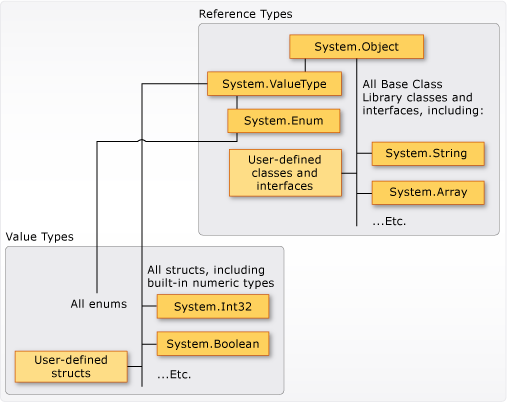
\includegraphics[width=140mm, height=100mm]{../img/value-reference-types-common-type-system}
%\caption{C\# type system \cite{online:cSharpTypeSystem}.}
%\label{img01:typeSystem}
%\end{figure}

\section{Roslyn}

\change{Overview of compilation pipeline}
\change{Binder}
\change{OverloadResolution}
\change{MethodTypeInferrer}
\change{NullableWalker}
\change{Dynamic biding vs. runtime binding}

\section{Hindley-Millner type inference}

\change{Hindley-Millner type system}
\change{Set of rules}
\change{Restriction and possible extensions}

\section{Rust type inference}

\change{Rust type system}
\change{Type inference context}
\change{Type inference across multiple statement}
\change{Constructor type inference}

\section{Github issues}

\change{Mention related Github issues and csharplang repo.}
\change{Roslyn and csharplang repo}
\change{Proposal champions}
\change{Related issues}

\chapter{Problem analysis}
\info{Describe the chapter}
The chapter divides the analysis into four sections. 
The first section describes the scope of the improvement based on the mentioned championed issue recommended by \ac{LDT}. 
The second section mentions a concrete motivation which leads us to the proposed improvement. 
The third section determines requirements based on the motivation, requirements given by proposing new language features, and Roslyn implementation internals. 
The fourth section describes the proposed language feature design, which is inspired by C\# language feature ideas mentioned in the previous chapter and validated by the requirements.
The last section mentions type inference improvements, whose implementation and proposal is not in the scope of this text, altought their possible implementation is sketched for being inspiration of future improvements. 

\section{Scope}
\info{Describe why we choose only a small part of the C\# type inference}
The previous chapter indicates that type inference is a complicated process, where even the current C\# method type inference is difficult to understand. 
Hence, the thesis chooses a small part of C\# where it improves and introduces the type inference and would be possible to reason about and implement in the scope of this text. 
The second reason for choosing a minor change is that introducing a completely new type inference in C\# would rather have an experimental result, which would have a smaller chance of getting into production, which is different from the intention of this work. 
However, some more extensive changes in the type inference will also be mentioned to outline possible obstacles to introducing them in the C\#.
\par
\info{Specify the focus on partial type inference}
The thesis focuses on the already-mentioned \textit{partial type inference} proposal, which was recommended by a member of \ac{LDT} and has a chance to be discussed in \ac{LDM} and potentially accepted. 
Analysis of this improvement contains a consideration of existing ideas, their consequences on C\#, and their difficulties in implementing them in Roslyn. 
Additionally, the work describes the relation to the Hindley-Millner formalization to express the strength of the type inference in a formalized way, which can be further used to compare it with other kinds of type inference in different programming languages and which decides the theoretical boundaries of the C\# type inference.

\section{Motivation}
\info{What is partial type inference and why it is useful}
Partial type inference focuses on hinting to the compiler ambiguous type arguments of generic type or method in situations where it can’t deduce them. 
In the context of C\#, the only type inference that infers type arguments is the method type inference mentioned in the previous chapter. 
The weakness of the method type inference is the need to provide hints to the compiler. 
The following three real-world examples demonstrate common issues with method type inference weakness, which the thesis tries to solve.
\par
\info{Weakness of current method type inference - target typing}
The first weakness regards target typing, which was mentioned in the previous chapter. 
Suppose a hypothetical situation when a user queries an item from a database whose column is a point of interest. 
Figure \ref{img27:usecase1} shows an example of code that uses the \texttt{fetch} method defined on a database type. 
The \texttt{data} variable represents data fetched from a database. 
Since a concrete form of data is unknown, the data has the type of \texttt{object} containing an internal representation of fetched data with the columns stored as fields. 
The \texttt{GetField} method enables one to read the variable’s field of the given name with the supposed type given as a type argument. 
Suppose the fetched object contains the ”name” field containing a string value. 
Now, a user wants to store the value in the \texttt{name} variable, which is explicitly typed. 
Even though the return type of the \texttt{GetField} method is known from the variable declaration, which also is the \texttt{TReturn} type argument of the method, the user still has to specify the type argument in the call. 
Generally, this problem consists of all type inferences, which depend on the target type. The target can be an argument of another method call or an assigning field. 
If the method type inference considers the target type, the user will not have to specify the \texttt{string} type argument in the \texttt{GetField} call.
\begin{figure}[h]
\begin{lstlisting}[style=csharp]
object data = database.fetch();
string name = data.GetField<string>("name");
...
static class Extensions {
    static 
    TReturn GetField<TReturn>(this object inst, string fieldName) 
    {...}
}
\end{lstlisting}
\caption{Target-typed inference.}
\label{img27:usecase1}
\end{figure}
\par
\info{Weakness of current method type inference - Constraints-based inference}
The second weakness is noticeable in more advanced generic APIs, like testing frameworks, using type constraints containing the type parameters. 
Figure \ref{img28:usecase2} shows a scenario of a simple test framework that defines the \texttt{Test} method parameterized by a type of input data and test case represented as type parameters \texttt{U} and \texttt{V}, respectively. 
The providing type argument representing the test case has to inherit the \texttt{TestCaseBase} base implementation, which is a generic type parametrized by a type of input data. 
This constraint gives type information about the \texttt{T} type parameter, which is related to the type of input data. 
However, the user has to specify type arguments in the \texttt{Test} call since the type inference doesn’t consider this source of type information. 
If the compiler considers the constraint, the type arguments will be inferred, saving the type annotations.
\begin{figure}[h]
\begin{lstlisting}[style=csharp]
Test<TestCaseBase<MyData>, MyData>(new MyData());
...
void Test<T, U>(U data) where T : TestCaseBase<U> {...}
\end{lstlisting}
\caption{Constraints-based inference.}
\label{img28:usecase2}
\end{figure}
\par
\info{Weakness of current method type inference - all or nothing principle}
There are also situations where even strong type inference is not enough.
Figure \ref{img29:usecase3} shows a situation where the \texttt{log} method is parametrized by two type parameters that are obtained in the parameter types and hence inferable by the compiler. 
However, the \texttt{log} method call still has to specify type arguments because the \texttt{null} argument doesn’t have concrete type information. 
In this case, the user always has to specify the second type argument, but the compiler can infer the first type argument. 
The thesis refers to this problem as \textit{all or nothing} principle, which regards the obligation to specify all type arguments or none of them.
\begin{figure}[h]
\begin{lstlisting}[style=csharp]
log<Message, Appendix>(new Message(...), null);
...
void log<T, U>(T message, U appendix) {...}
\end{lstlisting}
\caption{Uninferable type argument.}
\label{img29:usecase3}
\end{figure}
\par
\info{Breaking changes - Possible improvement of method type inference}
The first and the second weaknesses motivate us to extend the method type inference in order to consider a wider context for obtaining type information for the type arguments. 
This potential improvement is a problem for the compiler's back compatibility which was mentioned in the C\# discussion \cite{online:breakingChange}. 
New compiler versions should be back-compatible so that a new version does not change the behavior of the code compiled by the older version.
\par
\info{Breaking changes - target-typing}
Figure \ref{img30:breakingChange1} shows the breaking change when method type inference starts to consider target types. 
Before the improvement, the \texttt{M} method call is resolved to the non-generic version of this method because type inference can’t infer the \texttt{T} type argument. 
After the improvement, the type inference infers \texttt{T} to be the \texttt{int} type, which is more specific to the type of \texttt{1} argument than the \texttt{long} type. 
So now, the \texttt{M} method call refers to the generic version of this method and executes different code without any warning or error.
\begin{figure}[h]
\begin{lstlisting}[style=csharp]
int name = M(1);
...
T M<T>(int p1) {...}
int M(long p2) {...}
\end{lstlisting}
\caption{Breaking change: Target-typed inference.}
\label{img30:breakingChange1}
\end{figure}
\par
\info{Breaking changes - Constraints-based inference}
Figure \ref{img31:breakingChange2} shows a similar situation when the method type inference starts to consider type parameter constraints. 
Before the improvement, the \texttt{M} method call refers to the non-generic version of the method since the type inference can’t infer the type argument of a generic version. 
After the improvement, the generic version is inferred to have the \texttt{int} type argument and becomes to be more suitable for the overload resolution. 
So, the code behavior changed again because of compiling it with a different compiler's version.
\begin{figure}[h]
\begin{lstlisting}[style=csharp]
M(1);
...
void M<T>(int p1) where T : List<int> {...}
void M(long p2) {...}
\end{lstlisting}
\caption{Breaking change: Constraints-based inference.}
\label{img31:breakingChange2}
\end{figure}
\par
\info{Possible method type inference improvement doesn't solve the third weakness}
Besides the breaking change, the potential method type inference improvement to use a bigger context still doesn’t solve our third example demonstrating a type parameter, which doesn’t appear in parameter types, return type, and the type parameters’ constraints. 
These obstacles give the reason for introducing a way to hint just ambiguous type arguments to the compiler.
\par
\info{Partial type inference - reduces the first and second weakness}
Partial type inference can reduce the first two weaknesses. 
Type arguments, which the method type inference can’t infer, can be hinted in order to avoid specifying the whole type argument list. 
Let’s now ignore why the underscore character is used and how inferred type variables are determined in the following example. 
The reasons behind that will be mentioned later.
Figure \ref{img32:sol1} shows the usage of partial type inference applied in the second presented example regarding method type inference weaknesses. 
Although the first type argument of the \texttt{Test} method call must still be provided, the second argument is omitted by using the underscore character to determine an inferred type argument. 
The reduction of the first weakness is to isolate the insufficient type inference to type arguments that are directly influenced by it and infer the rest.
\begin{figure}[h]
\begin{lstlisting}[style=csharp]
test<TestCaseDefault<MyData>, _>(new MyData());

void test<T, U>(U data) where T : TestCaseDefault<U> {...}
\end{lstlisting}
\caption{Partial type inference: Reducing method type inference weakness.}
\label{img32:sol1}
\end{figure}
\par
\info{Breaking changes - solves the third weakness}
The third motivation example confirms that partial type inference is not just a fix for missing type inference features but is needed when type arguments can’t be inferred at all. 
Figure \ref{img33:sol2} demonstrates a usage of partial type inference where it omits the first type argument since it can be deduced from the first argument type and specifies the ambiguous type that can’t be deduced.
\begin{figure}[h]
\begin{lstlisting}[style=csharp]
log<_, Appendix>(new Message(...), null);

void log<T, U>(T message, U appendix) {...}
\end{lstlisting}
\caption{Partial type inference: Solving the \textit{all or nothing} problem.}
\label{img33:sol2}
\end{figure}
\par
\info{Constructor type inference - next motivation and improvement}
Partial type inference doesn’t regard only method type inference. 
It can also be introduced in other places. One of the places that seems to be good for that is object creation expression. 
Except for the already mentioned \texttt{new()} operator, no other type inference infers type arguments of a construing generic type. The usage of the type inference is limited since the \texttt{new()} operator requires a target type to infer the construing type. 
Figure \ref{img34:wrapper} shows an example of the limitation, where the \texttt{new()} operator can’t be used since the \texttt{IWrapper} target type is not the \texttt{Wrapper<int>} construing type. 
Hence, the user has to specify the whole type with the \texttt{int} type argument, despite the fact that it could be inferred using method type inference.
\begin{figure}[h]
\begin{lstlisting}[style=csharp]
IWrapper a = new Wrapper<int>(1);

class Wrapper<T> : IWrapper { public Wrapper(T item) {...} }
\end{lstlisting}
\caption{C\# wrapper class.}
\label{img34:wrapper}
\end{figure}
\par
\info{Constructor type inference - Factory method workaround}
In principle, object creation can be considered a special case of a method call with a side effect(creating the object), which already has method type inference. 
Figure \ref{img35:workaroung} shows a workaround using the \texttt{Create} method, delegating the creation to the constructor call. 
Since the method call type arguments can be inferred, it allows the use of method type inference for inferring type arguments of construing type. 
However, this solution has disadvantages like the necessary boiler-plate and prohibition of using initializers.
\begin{figure}[h]
\begin{lstlisting}[style=csharp]
IWrapper a = Create(1);

static Wrapper<T> Create<T>(T item) => new Wrapper<T>(item);
\end{lstlisting}
\caption{Workaround of constructor type inference.}
\label{img35:workaroung}
\end{figure}
\par
\info{Constructor type inference - strength of method type inference}
A possible solution would be to use method type inference in object creation expression. 
Although this solution would be simple to implement, class type parameters are more likely not to be used in constructor parameter types, which makes the method type inference useless. 
Besides that, options for inferring type arguments of construing type are not limited by not introducing breaking changes since there is no type inference at all. 
So, there is a possibility of introducing an even stronger type inference, which could be one day introduced in the method type inference when there would be a way to make breaking changes in the new compiler version. 
Figure \ref{img36:cti} shows an example of such a generic class whose all type parameters are not used in the constructor.
Because of that, extending the potential method type inference to be used in object creation expressions would be useless since the \texttt{TLogger} can’t be inferred only from parameter types.
\begin{figure}[h]
\begin{lstlisting}[style=csharp]
class Algorithm<TData, TLogger> where TLogger : Logger<TData> 
{ public Algorithm(TData data) { ... }}
\end{lstlisting}
\caption{Use case iusing type paraemter constraints.}
\label{img36:cti}
\end{figure}
\par
\info{Constructor type inference - the first weakness solution}
Introducing improved type inference based on method type inference would solve the mentioned issues. 
Figure \ref{img37:sol1} shows a potential usage of that type inference in the first case regarding the Wrapper class where an underscore is used to represent inferred type argument. 
The inference uses the parameter type of the constructor to infer the \texttt{T} parameter type which is \texttt{int}.
\begin{figure}[h]
\begin{lstlisting}[style=csharp]
IWrapper a = new Wrapper<_>(1);

class Wrapper<T> : IWrapper { public Wrapper(T item) {...} }
\end{lstlisting}
\caption{Constructor type inference: Wrapper.}
\label{img37:sol1}
\end{figure}
\par
\info{Constructor type inference - better method type inference}
Figure \ref{img38:sol2} shows a potential improvement of the type inference. 
The first statement of initializing the \texttt{alg} variable uses type inference, leveraging \texttt{TLogger}’s constraint to determine its type. 
The second statement demonstrates the possibility of having a nested underscore, which allows to more specify the type argument.
\begin{figure}[h]
\begin{lstlisting}[style=csharp]
var alg = new Algorithm<_, _>(new MyData());
var algWithSpecialLogger = 
    new Algorithm<_ , SpecialLogger<_>>(new MyData());

class Algorithm<TData, TLogger> 
    where TLogger : Logger<TData> 
{ public Algorithm(TData data) { ... }}
\end{lstlisting}
\caption{Constructor type inference: stronger method type inference.}
\label{img38:sol2}
\end{figure}
\par
From now on, thesis calls \textit{constructor type inference} for introducing such a type inference.

\section{Requirements}

\info{intro}
This section mentions requirements that have to be fulfilled by the improvement to be likely discussed by \ac{LDM}.
\par
\info{Describe requirements given by back compatibility}
\textbf{Back compatibility} is one of the most important requirements for new language features. 
The improvement shouldn’t introduce a breaking change. However, this requirement is sometimes too strict for improvements, which would be very beneficial, and its breaking change would appear in cases that seem to be rare in the code. 
These improvements can break back compatibility by providing additional warnings or errors alerting a user of possible code behavior changes.
Figure \ref{img39:brkCh} shows an introduced breaking change when record classes were added into the C\# language. 
Before the change, the \texttt{B} identifier referred to a method without parameters and returning the \texttt{record} type. 
After the change, the \texttt{B} identifier refers to a new record type declaration. 
There is an example where the breaking change can appear when there is a type with the \texttt{record} name. 
These situations are uncommon, and the improvement benefit was big enough to be added to the language. 
The possible breaking change is notified to the user by a compilation error.
\begin{figure}[h]
\begin{lstlisting}[style=csharp]
class record {}
class A {
    record B(){...}
}
\end{lstlisting}
\caption{C\# record class breaking change.}
\label{img39:brkCh}
\end{figure}
\par
\info{Decribe requirements given by motivation}
\textbf{Convenience} is a key requirement to make the improvement useful. 
Regarding partial type inference, the improvement should propose a convenient way to skip ambiguous type arguments. 
The way should also be possible to use in different places where skipping type arguments could yield an advantage, like type variable declaration or casting to a different type. 
Constructor type inference should be advanced enough to cover the mentioned examples.
\par
\info{Describe requirements given by Future improvements}
\textbf{Extensibility} would make the improvement open for new features that can be needed in future language versions. 
The improvement should consider possible future improvements and not be a blocker for them.
\par
\info{Describe requirements given by Roslyn}
\textbf{Performance} is a critical section of Roslyn, which is one of the main goals of this project.
The time complexity added by the thesis’s improvement shouldn’t be too big in order to not slow the compilation process.

\section{Language feature design}

\info{Intro}
This section describes the language design of the proposed improvement.
It discusses existing ideas of the partial type inference, and combines them to form the proposed design.
Than, it adjusts method type inference algorithm to handle partially defined type arguments and introduces constuctor type inference extending method type inference.
\par
\info{Discuss mentioned ideas}
Mentioned ideas can be categorized into 3 groups.
The first group consists of target-typed inference and type inference based on type constraints which improve method type inference algorithm.
The second group consists of default type parameters, generic aliases, named type parameters, using char as inferred type argument, and realocation which reagrds partial type inference.
the third group consists of constructor type inference and type inferecne of method return type which introduce type inference in new C\# constructs.
Method return type inference is not in the scope of this work, although it is mentioned in the next section as a future improvement which will be difficult to implement.
The first group is discussed in relation to constructor type inference where pottentially applied method type inferance can be improved without introducing breaking changes.
The second group is discussed in relation to partial type inference which is an objective of the campioned issue.

\subsection{Partial method type inference}

Discussions regarding partial type inference can be further divided into two groups.
The first group provides the hints in type parameter declarations which is done by default type parameters.
Since it has to be done in the declaration, partial type inferenec wouldn't work with already existing code without adjusting it.
For this reason, the work excludes the idea.
\par
The second group provides the hints through the usage.
Generic aliases doesn't work for methods and also it doesn't seem to be useful when the inferred type arguments doesn't represent some common specialization of generic type which can be used example of \texttt{StringDictionary<TValue>}.
\par
Named type parameters are excluded since providing that woudl be uncommon new feature which has no equivalent in other well-known languages like Java, C++, Kotlin, and Rust.
We believe it would be confusing to introduce it to the users since it is controversial change.
\par
Realocation doesn't sovle the problem with specifying all type arguments and it just compacts type argument lists into one.
\par
The last discussing regards unsing char as inferred type argument which is a core of the proposed design for the following reasons.
It is already used in different languages like a star in Kolin and Java or an underscore in Rust and F\#.
So it is more common and intentional then previously mentioned ideas.
It introduces no or at least minimal syntax changes into the language which makes the usage simple.
And it sovles the the problem with specifying all type arguments.

\subsubsection{Choosing the syntax}

The choice of the syntax is based on five use cases where the expression of inferred type argument can be used or could be used in the future.
Table \ref{table2:useCasesChar} shows examples of these usages which identify necessary requirements on the syntax.
\begin{table}[h]
\begin{center}
\begin{tabular}{ | l | c | } 
  \hline
  Generic method call & \texttt{Foo<\{SYNTAX\}>(arg1, arg2,...)}\\
  \hline
  Object creation expression & \texttt{new Bar<\{SYNTAX\}>(arg1, arg2,...)}\\
  \hline
  Variable declaration & \texttt{Bar<\{SYNTAX\}> temp = ...}\\
  \hline
  Array type & \texttt{\{SYNTAX\}[]}\\
  \hline
  Inferred type & \texttt{\{SYNTAX\}}\\
  \hline
\end{tabular}
\end{center}
\caption{Use cases containing syntax for inferred type argument.}
\label{table2:useCasesChar}
\end{table}
\par
\textbf{Generic method call} use case represents a situation where the syntax is used during a generic method call.
\par
\textbf{Object creation expression} represents the usage in construction of generic type.
\par
\textbf{Variable declaration} represents the potential usage in variable type declaration which is not in the scope of this work, however it is natural continuation of partial type inference extension where the inferred type arguments are deremined by the surrounding context.
\par
\textbf{Array type} has a different syntax of type argument list specifying a type of the contained elements.
The type of the elements can be also inferred and the proposed syntax has to offer convenient way how to express an array type with the inferred element type.
\par
\textbf{Inferred type} doesn't have to be contained only in the type argument list.
The previous chapter presented the \text{var} keyword used in the variable declaration whose type is determined by the type of initializing value.
C\# also offers a discard pattern \cite{online:discard} represented by an underscore which is commonly used as placeholders for variables which are not intentionally used in the code.  
Since type argument inference relates to that, the syntax should be at least aligned with already existing related syntax.
The allignment will help the syntax to be naturally used without using a language documentation.
\par
There are several syntax which can be used for inferred type.
The work presents the most relavent syntax which appeared in the mentioned ideas and comments on advantages and disadvantages for the each of them.

\paragraph*{Diamond operator} is represened by pair of two angle brackets \texttt{<>}.
It is used as empty type argument list determining that the type name or method name is generic.
\par
Figure \ref{img40:opDi1} demonstrates the usage in generic method calls of \texttt{Foo1} and \texttt{Foo2}.
The declarations of these methods are not important for the purpouse of showing pros and cons.
Calling the \texttt{Foo1} method with an empty argument list doesn't much make sense since method type inference is enabled by default without using angle brackets.
Calling the \texttt{Foo2} method with nested usage of diamond operator allows limited partial type inference when the diamond operator is used inside the type argument list.
The \texttt{Bar<>} type partially hint the compiler the generic type name without specifying the type arguments.
However, the usage is problemeatic when there is multiple generic types with the same name since it can cause ambiguity between them.
This problem is described in the next example.
\begin{figure}[h]
\begin{lstlisting}[style=csharp]
Foo1<>(arg1, arg2, arg3);
Foo2<Bar<>, int>(arg1, arg2, arg3);
\end{lstlisting}
\caption{Diamond operator - generic method call.}
\label{img40:opDi1}
\end{figure}
\par
Figure \texttt{img41:opDi2} shows the usage in object creation expression.
The first statement containing \texttt{Bar<>} name has an advantage of expressing the will to infer the type's type arguments which is necessary in comparison the previous example since the object creation doesn't offer type inference.
If the type inference would be potentially turned on by default, it would introduce a breaking change.
Alhought, there is also an disadvantage of the usage since it doesn't specify the arity of the generic type.
If there would be multiple generic types diferring in arity, it would complicate the already mentioned overload resolution phase since all constructors from these generic types would have to be considered.
The process would be computationally demanding.
Possible solution would be the following restriction. 
Usually, there is not more than one generic type with the same name. 
So when there will be just one type of that name, the diamond operator would be allowed to use since it determined one specific generic type.
In the example, \texttt{Baz<>} would refer to \texttt{Baz<T1, T2>} generic type since there is no other generic type with the same name causing the ambiguity.
\begin{figure}[h]
\begin{lstlisting}[style=csharp]
new Bar<>(...);
new Baz<>(...);

class Bar { ... }
class Bar<T1> { ... }
class Bar<T1, T2> { ... }

class Baz<T1,T2> { ... }
\end{lstlisting}
\caption{Diamond operator - object creation expression.}
\label{img41:opDi2}
\end{figure}
\par
The third example is shown in Figure \ref{img42:opDi3}, where the generic \texttt{Wrapper} class is used to specify the wrapping generic type.
However, it doesn't offer to specify any type arguments which is limiting when the compiler can't infer all of them..
\begin{figure}[h]
\begin{lstlisting}[style=csharp]
Wrapper<> temp = ...
\end{lstlisting}
\caption{Diamond operator - variable declaration.}
\label{img42:opDi3}
\end{figure}
\par
Figure \ref{img43:opDi4} shows the operator as a indicator of inferred element of the array type.
Since there isn't known popular language similar to C\# which would contain the similar construct, the usage is considered to be unintentiaonal for the most of the users.
\begin{figure}[h]
\begin{lstlisting}[style=csharp]
<>[] temp = ...
\end{lstlisting}
\caption{Diamond operator - array type.}
\label{img43:opDi4}
\end{figure}
\par
The similar conslusions are made in the last example in Figure \ref{img44:opDi5} where the \texttt{<>} operator has the same functionality as already existing \texttt{var} keyword.
\begin{figure}[h!]
\begin{lstlisting}[style=csharp]
<> temp = ...
\end{lstlisting}
\caption{Diamond operator - inferred type.}
\label{img44:opDi5}
\end{figure}

\paragraph*{Whitespace seperated by commas} is the next proposing syntax which would allow to skip inferred type arguments and specify just the amigious.
It would also determine the arity of type which is important for the type name look up phase of the compiler.
Natural choice for the separator is commas since it is widely used.
Another advantage is that this syntax is already used when working with C\# reflaction.
An example is the following expression \texttt{typeof(Dictionary<,>)} which returns a class describing the \texttt{Dictionary} type.
\par
Figure \ref{img45:opW1} shows the usage when the \texttt{Foo1} generic method is called with skipping the first and the last type argument which is inferred by the compiler.
However, the syntax seems to be messy when it is used in generic methods with many generic type parameters as can be seen in the \texttt{Foo2} method call.
The similar thoughs regard the second and third use case.
\begin{figure}[h]
\begin{lstlisting}[style=csharp]
Foo1<, string, List<>, >(arg1, arg2, arg3);
Foo2<,,,int,,>(arg1, arg2, arg3);
\end{lstlisting}
\caption{Whitespace - generic method call.}
\label{img45:opW1}
\end{figure}
\par
The usage with array type seems to be unintantianal and would caused changes in the compiler parser. 
Figure \ref{img46:opW4} shows the syntax to express inferred type of array's element. 
\begin{figure}[h]
\begin{lstlisting}[style=csharp]
[] temp = ...
Foo<, [], >(arg1, arg2)
\end{lstlisting}
\caption{Whitespace - array type.}
\label{img46:opW4}
\end{figure}
\par
The last use case regarding using the whitespace as a inferred type would probable caused problems with determining declarations of variables.
Figure \ref{img47:opW5} shows a situation where the compiler can't determine if it is a variable declaration or an variable assignment.
Although it could be solved by investigating surronding context, we consider that the code comprehension would get worse.
\begin{figure}[h]
\begin{lstlisting}[style=csharp]
temp = ...
\end{lstlisting}
\caption{Whitespace - inferred type.}
\label{img47:opW5}
\end{figure}

\paragraph*{Underscores seperated by commas} is commonly used in other programming languages like F\# or Haskell to represent inferred type arguments or as a placeholder for discarding variables wich are intentianolly not used.
This is considered as a big advantage.
An disadvantage is the introduction of breaking change because C\# allows the underscore as a type identifier.
However, that seems to be rather uncommon in the code. 
It seems to be less messy then previous syntax when a generic type contains many type parameters as it is shown in Figure \ref{img50:opU1}.
\begin{figure}[h!]
\begin{lstlisting}[style=csharp]
new Bar<_, _, List<_>, _,_>(arg1, arg2, arg3);
\end{lstlisting}
\caption{Underscore - object creation expression.}
\label{img50:opU1}
\end{figure}
\par
The usage with array type also seems to work even it can be still considered uncommon.
Figure \ref{img51:opU4} shows the usage where we think that the syntax intentianally express the inferred type of array's elements.
\begin{figure}[h!]
\begin{lstlisting}[style=csharp]
_[] temp = ...
\end{lstlisting}
\caption{Underscore - array type.}
\label{img51:opU4}
\end{figure}
\par
The last use case is shown in Figure \ref{img52:opU5} where it clashes with already existing \texttt{var} keyword.
\begin{figure}[h!]
\begin{lstlisting}[style=csharp]
_ temp = ...
\end{lstlisting}
\caption{Underscore - variable declaration.}
\label{img52:opU5}
\end{figure}

\paragraph*{\texttt{var} keywords seperated by commas} are another natural option of the syntax.
The big advantage of the syntax is already used \texttt{var} keyword in the variable declaration which meaining is coherent with inferred type arguments.
However, it starts to raise the question if it brings the advantage of saving keystrokes.
Figure \ref{img52:opV1} shows an usage of the syntax which is considered to be unnecessary long.
\begin{figure}[h]
\begin{lstlisting}[style=csharp]
Foo<var, string, List<var>, int>(arg1, arg2, arg3);
\end{lstlisting}
\caption{\texttt{var} - generic method call.}
\label{img52:opV1}
\end{figure}

\paragraph*{Something else seperated by commas} doesn't make a lot of sense because it needs to assign new meaning to that character in comparison with an underscore, the \texttt{var} keyword, the \texttt{<>} operator, or \texttt{<,,,>} syntax. An asterisk can be considered, however, it can remind a pointer in the context of unmanaged C\# code.

\paragraph*{Conslusion} The thesis chooses the underscore as a placeholder for inferred type argument since the meaning of this character it related to the intention.
It also seems to be the shortest and synoptical way how to skip inferred type arguments.
Possible breaking change is not a obstacle in this situation since the similar decision was made for the \texttt{var} keyword and the situation where it can occurs seem to be rare.
Problems with the potential future extension where the underscore can represent inferred type in variable declaration would be prohibit to not mix it with the \texttt{var} keyword.
Although the diamond operator is not very useful in generic method call, it makes sence in object creation expression.
The usage and analysis of that is covered by this work as well.

\subsubsection{Method lookup}

TODO

\subsubsection{Method type inference algorithm change}

TODO

\subsection{Partial constructor type inference}

TODO

\subsubsection*{Class lookup}

TODO

\subsubsection*{Constructor type inference}

TODO

\subsubsection*{Initiliazers extension}

TODO

\subsubsection*{Diamond operator extension}

TODO

\change{Explain why they fullfill the requirements}

TODO

\section{Other type inference improvements}

TODO

\change{Shared type inference context}

TODO

\change{Inferring return value of methods}

TODO
\chapter{Solution}


\change{Describe process of making proposal and the prototype.}
\change{Describe partial method type inference.}
\change{Describe constructor type inference.}
\change{Describe generic adjusted algorithm for type inference.}
\change{Describe decisions of proposed change design.}
\change{Describe changed parts of C\# standard.}
\chapter{Evaluation}

\change{Describe achieved type inference. Mention interesting capabilities.}
\change{Note about the performance.}
\change{Links to csharplang discussions.}
\chapter{Future improvements}

\change{Mention next steps which can be done.}
\change{Discuss which steps would not be the right way(used observed difficulties).}

\chapter*{Conclusion}
\addcontentsline{toc}{chapter}{Conclusion}

The introduction \ref{sect:summary} sets four goals, which are gradually achieved by the thesis. 
It starts by exploring C\# type inference by using the language specification and implementation in the Roslyn project. 
Then, it compares with Rust type inference, which offers more advanced type inference than C\#. 
These differences are explained using the theory background of Hindley-Milner type inference, which describes the limits of type inference in strongly typed languages.
\par
Based on these observations, the work selects a subset of type inference improvements suggested in C\# language discussions on GitHub and explores the motivation behind it to make it likely to add to C\# language. 
The motivation is described in the created proposal, which is the fourth goal and which describes the improvement in terms of changing the specification.
\par
Together with the proposal, the implementation was made in the Roslyn project fork, with unit tests checking the functionality. 
This was the last goal of the proposal. 
The implementation ensured that basic compiler tests passed to reveal possible issues with the solution.
\par
In addition to the mentioned goals, the thesis succeeded in presenting the proposal and implementation to the \ac{LDM} responsible for approving language changes into C\#. 
The committee agreed to continue with the change for further discussion and is generally inclined to ship it with future language releases.
\par
Based on the goals achieved and additional success in the \ac{LDM} meeting, which was not a part of the scope of the work, we think that the thesis accomplished all the promised goals.


%%% Bibliography
%%% Bibliography (literature used as a source)
%%%
%%% We employ bibTeX to construct the bibliography. It processes
%%% citations in the text (e.g., the \cite{...} macro) and looks up
%%% relevant entries in the bibliography.bib file.
%%%
%%% The \bibliographystyle command selects, which style will be used
%%% for references from the text. The argument in curly brackets is
%%% the name of the corresponding style file (*.bst). Both styles
%%% mentioned in this template are included in LaTeX distributions.

\bibliographystyle{plainnat}    %% Author (year)
% \bibliographystyle{unsrt}     %% [number]

\renewcommand{\bibname}{Bibliography}

%%% Generate the bibliography. Beware that if you cited no works,
%%% the empty list will be omitted completely.

\bibliography{bibliography}

%%% If case you prefer to write the bibliography manually (without bibTeX),
%%% you can use the following. Please follow the ISO 690 standard and
%%% citation conventions of your field of research.

% \begin{thebibliography}{99}
%
% \bibitem{lamport94}
%   {\sc Lamport,} Leslie.
%   \emph{\LaTeX: A Document Preparation System}.
%   2nd edition.
%   Massachusetts: Addison Wesley, 1994.
%   ISBN 0-201-52983-1.
%
% \end{thebibliography}


%%% Figures used in the thesis (consider if this is needed)
\listoffigures

%%% Tables used in the thesis (consider if this is needed)
%%% In mathematical theses, it could be better to move the list of tables to the beginning of the thesis.
\listoftables

%%% Abbreviations used in the thesis, if any, including their explanation
%%% In mathematical theses, it could be better to move the list of abbreviations to the beginning of the thesis.
\chapwithtoc{List of Abbreviations}
\begin{acronym}
 \acro{LDM}{Language Design Team}
 \acro{CTS}{Common Type System}
 \acro{CIL}{Common Intermediate Language}
\end{acronym}

%%% Attachments to the master thesis, if any. Each attachment must be
%%% referred to at least once from the text of the thesis. Attachments
%%% are numbered.
%%%
%%% The printed version should preferably contain attachments, which can be
%%% read (additional tables and charts, supplementary text, examples of
%%% program output, etc.). The electronic version is more suited for attachments
%%% which will likely be used in an electronic form rather than read (program
%%% source code, data files, interactive charts, etc.). Electronic attachments
%%% should be uploaded to SIS and optionally also included in the thesis on a~CD/DVD.
%%% Allowed file formats are specified in provision of the rector no. 72/2017.
\appendix
\chapter{Attachments}

\openright
\end{document}
